
\documentclass[journal,12pt,twocolumn]{IEEEtran}

\usepackage{setspace}
\usepackage{gensymb}

\singlespacing


\usepackage[cmex10]{amsmath}

\usepackage{amsthm}

\usepackage{mathrsfs}
\usepackage{txfonts}
\usepackage{stfloats}
\usepackage{bm}
\usepackage{cite}
\usepackage{cases}
\usepackage{subfig}

\usepackage{longtable}
\usepackage{multirow}

\usepackage{enumitem}
\usepackage{mathtools}
\usepackage{steinmetz}
\usepackage{tikz}
\usepackage{circuitikz}
\usepackage{verbatim}
\usepackage{tfrupee}
\usepackage[breaklinks=true]{hyperref}
\usepackage{graphicx}
\usepackage{tkz-euclide}

\usetikzlibrary{calc,math}
\usepackage{listings}
    \usepackage{color}                                            %%
    \usepackage{array}                                            %%
    \usepackage{longtable}                                        %%
    \usepackage{calc}                                             %%
    \usepackage{multirow}                                         %%
    \usepackage{hhline}                                           %%
    \usepackage{ifthen}                                           %%
    \usepackage{lscape}     
\usepackage{multicol}
\usepackage{chngcntr}

\DeclareMathOperator*{\Res}{Res}

\renewcommand\thesection{\arabic{section}}
\renewcommand\thesubsection{\thesection.\arabic{subsection}}
\renewcommand\thesubsubsection{\thesubsection.\arabic{subsubsection}}

\renewcommand\thesectiondis{\arabic{section}}
\renewcommand\thesubsectiondis{\thesectiondis.\arabic{subsection}}
\renewcommand\thesubsubsectiondis{\thesubsectiondis.\arabic{subsubsection}}


\hyphenation{op-tical net-works semi-conduc-tor}
\def\inputGnumericTable{}                                 %%

\lstset{
%language=C,
frame=single, 
breaklines=true,
columns=fullflexible
}
\begin{document}


\newtheorem{theorem}{Theorem}[section]
\newtheorem{problem}{Problem}
\newtheorem{proposition}{Proposition}[section]
\newtheorem{lemma}{Lemma}[section]
\newtheorem{corollary}[theorem]{Corollary}
\newtheorem{example}{Example}[section]
\newtheorem{definition}[problem]{Definition}

\newcommand{\BEQA}{\begin{eqnarray}}
\newcommand{\EEQA}{\end{eqnarray}}
\newcommand{\define}{\stackrel{\triangle}{=}}
\bibliographystyle{IEEEtran}
\providecommand{\mbf}{\mathbf}
\providecommand{\pr}[1]{\ensuremath{\Pr\left(#1\right)}}
\providecommand{\qfunc}[1]{\ensuremath{Q\left(#1\right)}}
\providecommand{\sbrak}[1]{\ensuremath{{}\left[#1\right]}}
\providecommand{\lsbrak}[1]{\ensuremath{{}\left[#1\right.}}
\providecommand{\rsbrak}[1]{\ensuremath{{}\left.#1\right]}}
\providecommand{\brak}[1]{\ensuremath{\left(#1\right)}}
\providecommand{\lbrak}[1]{\ensuremath{\left(#1\right.}}
\providecommand{\rbrak}[1]{\ensuremath{\left.#1\right)}}
\providecommand{\cbrak}[1]{\ensuremath{\left\{#1\right\}}}
\providecommand{\lcbrak}[1]{\ensuremath{\left\{#1\right.}}
\providecommand{\rcbrak}[1]{\ensuremath{\left.#1\right\}}}
\theoremstyle{remark}
\newtheorem{rem}{Remark}
\newcommand{\sgn}{\mathop{\mathrm{sgn}}}
\providecommand{\abs}[1]{\left\vert#1\right\vert}
\providecommand{\res}[1]{\Res\displaylimits_{#1}} 
\providecommand{\norm}[1]{\left\lVert#1\right\rVert}
%\providecommand{\norm}[1]{\lVert#1\rVert}
\providecommand{\mtx}[1]{\mathbf{#1}}
\providecommand{\mean}[1]{E\left[ #1 \right]}
\providecommand{\fourier}{\overset{\mathcal{F}}{ \rightleftharpoons}}
%\providecommand{\hilbert}{\overset{\mathcal{H}}{ \rightleftharpoons}}
\providecommand{\system}{\overset{\mathcal{H}}{ \longleftrightarrow}}
	%\newcommand{\solution}[2]{\textbf{Solution:}{#1}}
\newcommand{\solution}{\noindent \textbf{Solution: }}
\newcommand{\cosec}{\,\text{cosec}\,}
\providecommand{\dec}[2]{\ensuremath{\overset{#1}{\underset{#2}{\gtrless}}}}
\newcommand{\myvec}[1]{\ensuremath{\begin{pmatrix}#1\end{pmatrix}}}
\newcommand{\mydet}[1]{\ensuremath{\begin{vmatrix}#1\end{vmatrix}}}
\numberwithin{equation}{subsection}
\makeatletter
\@addtoreset{figure}{problem}
\makeatother
\let\StandardTheFigure\thefigure
\let\vec\mathbf
\renewcommand{\thefigure}{\theproblem}
\def\putbox#1#2#3{\makebox[0in][l]{\makebox[#1][l]{}\raisebox{\baselineskip}[0in][0in]{\raisebox{#2}[0in][0in]{#3}}}}
     \def\rightbox#1{\makebox[0in][r]{#1}}
     \def\centbox#1{\makebox[0in]{#1}}
     \def\topbox#1{\raisebox{-\baselineskip}[0in][0in]{#1}}
     \def\midbox#1{\raisebox{-0.5\baselineskip}[0in][0in]{#1}}
\vspace{3cm}
\title{Assignment-4}
\author{Ankur Aditya - EE20RESCH11010}
\maketitle
\newpage
\bigskip
\renewcommand{\thefigure}{\theenumi}
\renewcommand{\thetable}{\theenumi}

\begin{abstract}
This document contains the procedure to find value of $\sin60\degree$.
\end{abstract}
Download the python code from 
\begin{lstlisting}
https://github.com/ankuraditya13/EE5609-Assignment4
\end{lstlisting}
%
and latex-file codes from 
%
\begin{lstlisting}
https://github.com/ankuraditya13/EE5609-Assignment4
\end{lstlisting}

\section{Problem}
Show that $\sin60\degree = \frac{\sqrt{3}}{2}.$
\section{Solution}
Consider an equilateral triangle \textbf{ABC}. Since, $\triangle$\textbf{ABC} is an equilateral, all of its angles are $60\degree$. Now, The direction vector of all the sides are given as,
\begin{align}
\vec{AB}=\norm{\vec{A-B}}
\end{align}
\begin{align}
\vec{BC}=\norm{\vec{B-C}}
\end{align}  
\begin{align}
\vec{AC}=\norm{\vec{A-C}}
\end{align} 
Now for an equilateral triangle,
\begin{align}
\norm{\vec{A-B}} = \norm{\vec{B-C}} = \norm{\vec{A-C}}
\label{eq2}
\end{align}
In figure \ref{Fig 1}, taking inner products of side $\vec{AB}$ and $\vec{BC}$ we get,
\begin{align}
\vec{AB}\cdot\vec{BC} = \norm{\vec{AB}}\norm{\vec{BC}}\cos\theta
\label{eq3}
\end{align} 
Let, $ \vec{a} = \vec{A}-\vec{B}, \vec{b} = \vec{B}-\vec{C}$. Hence $\vec{A}-\vec{C} = \vec{a}+\vec{b}.\\\therefore$ the angle $\theta$ between two vectors  $\vec{AB}$ and $\vec{BC}$ is given by,
\begin{comment}
\begin{align}
\cos\theta  = \brak{\frac{\norm{\vec{a}}^2 + \norm{\vec{b}}^2 - \norm{\vec{a}+\vec{b}}^2}{2\norm{\vec{a}}\norm{\vec{b}}}}
\end{align}
\end{comment}
\begin{align}
\cos\theta = \frac{\vec{a}^T\cdot\vec{b}}{\norm{\vec{a}}\norm{\vec{b}}}
\end{align}
Substituting from equation \ref{eq2} to \ref{eq3} we get,
\begin{align}
\implies \cos\theta = \frac{1}{2}
\end{align}
we know that $\theta = 60\degree$ for an equilateral triangle 
\begin{align}
\therefore \cos60\degree = \frac{1}{2}
\end{align}
Now using the property,
\begin{align}
\cos^2\theta +\sin^2\theta = 1
\end{align} 
$\therefore$ at $\theta = 60\degree, $
\begin{align}
\sin60\degree = \sqrt{1-\cos^260\degree}
\end{align}
\begin{align}
\implies\sin60\degree = \frac{\sqrt{3}}{2}.
\end{align}
\begin{figure}
\centering
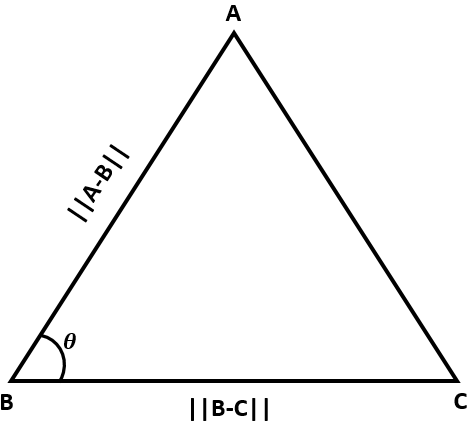
\includegraphics[width=\columnwidth]{a_4_2.png}
\caption{Equilateral Triangle}
\label{Fig 1}
\end{figure}
\end{document}